\documentclass[conference]{IEEEtran}

\usepackage{cite}
\usepackage{amsmath,amssymb,amsfonts}
\usepackage{algorithmic}
\usepackage{graphicx}
\usepackage{textcomp}
\usepackage{xcolor}
\def\BibTeX{{\rm B\kern-.05em{\sc i\kern-.025em b}\kern-.08em
    T\kern-.1667em\lower.7ex\hbox{E}\kern-.125emX}}
\begin{document}

\title{An Unending Battle:\\A Thorough Analysis of the RISC vs CISC Debate and a Verilog Simulation of the RISC Architecture\\
{\footnotesize \textsuperscript{*}Not an IEEE research paper. Done as part of a Computer Architecture Project}
}

\author{\IEEEauthorblockN{Kabir Kanha Arora}
\IEEEauthorblockA{\textit{Sophomore Year, Computer Science and Engineering} \\
\textit{Shiv Nadar University}\\
Greater Noida, India \\
ka682@snu.edu.in \\
\textbf{1710110165}}
\and
\IEEEauthorblockN{Komal Talwar}
\IEEEauthorblockA{\textit{Sophomore Year, Computer Science and Engineering} \\
\textit{Shiv Nadar University}\\
Greater Noida, India \\
kt252@snu.edu.in \\
\textbf{1710110183}}
}

\maketitle

\begin{abstract}
This paper revisits the unsettled battle for supremacy between RISC and CISC instruction sets, gives a thorough analysis and conclusion for the same, and finishes off with a verilog based simulation of the RISC microcontroller.
\end{abstract}

\begin{IEEEkeywords}
isa, risc, cisc, arm, computer, architecture, verilog, simulation
\end{IEEEkeywords}

\section{Introduction to ISA}
Instruction Set Architecture (ISA) is also known as CPU architecture. ISA allows communication between software and hardware. It is also a group of commands for CPU and machine language. So basically, ISA tells you how your processor is going to process your program's instructions. An instruction, just to clarify, is also known as op-code or operation code. Some examples of op-codes are \verb|ADD, JUMP, LOAD| and \verb|STORE|. 

Instruction set architecture serves as a bridge between the software and hardware layers of a computer system, binding the two by acting as a means of communication of the processor. It lists all the instructions that an operator can give. Among the components of an instruction set architecture, some of these are registers, addressing modes, data-types, memory management, devices and exception handling, power management and multi-threading support. The instructions that exist in the set are used to alter the machine state, data or are used for performing an I/O operation.

Most modern ISAs are classified into \textbf{RISC} (Reduced instruction set Computer) and \textbf{CISC} (Complex instruction set computer) on the basis of their architectural complexity.  Other architectures include \textit{VLIW, LIW and EPIC}. These are used to rely less on hardware and exploit instruction level parallelism. All these architectures vary in their complexity and the portion of the computer system that they are willing to exploit.
A study conducted, which focused on the effect of ISAs on code density, observed that code density is mostly affected by the number of registers being used, length of an instruction, hardware divisors, number of operands, etc. The study conjointly showed that x86 (which has CISC in use) is one of the densest ISAs. As another observation by experimentation, it has been seen that compression of immediate values in instructions gives us a \textbf{30\%} reduction in code size along with a significant \textbf{10\%} reduction in processor’s power consumption.

Several studies have concluded that RISC incorporates a performance edge over CISC processors and that CISC requires more aggressive microarchitecture optimizations to overcome the performance bottleneck. There exist other studies that say with time and rapid evolution in technology, the gap between RISC and CISC won’t matter as \textit{Moore’s law} starts to diminish.
Our study emphasizes on RISC and its simple differences with CISC. 


\section{The two types of ISA}

\subsection{Complex Instruction Set Computing (CISC)}

There are two types of ISA. The first one is \textbf{CISC}, which stands for \emph{Complex Instruction Set Computing}. It is an architecture with a large number of instruction sets. For instance, the microprocessor of CISC is Intel x64, which the 64-bit version of the x86 instruction set. They are mostly found in desktop and laptops. 

\subsection{Reduced Instruction Set Computing (RISC)}

Now, on the other hand, \textbf{RISC}, yes with a C, stands for \emph{Reduced Instruction Set Computing}, is another type of ISA which has a smaller set of instructions.\\
\textbf{For eg:} ARM processors are extensively used in consumer electronic devices such as tablets, smartphones and even gaming consoles. RISC is a form of microprocessor architecture that utilizes a small, highly-optimized set of instructions, instead of an additional specialised set of instructions often found in alternative types of architectures. 


\section{The Popularity of CISC}
Up until about the 1980s, most computer processors (the CPUs) were getting more and more complicated and the idea was that if you could make the hardware sort of mirror the software, then of course it would be quicker. So as you wrote a program (which was probably exclusively in \textit{C} or \textit{Fortran} in those days), it produced certain instructions. If those instructions could be executed more and more in the hardware with less and less instructions, that would make the whole thing go much faster. And obviously, there were also other considerations like memory being expensive and so if you had shorter programs, such that each instruction could do more complicated things and take up less space, that would be better. The speed of memory and the complexity of processes themselves was different, and so was the number of transistors involved.


\section{The emergence of RISC}
And then in the early 1980s, this idea came along of having a reduced complexity and that’s what got it its name. Although, as we’ll see later, it’s not really about having a smaller number of instructions, it’s more about how you use those instructions. Now, the argument was put forward like this by \textbf{David Patterson}, a renowned computer scientist and author:
\begin{quote}
\textit{“The simplicity of the instruction set and addressing modes allows most instructions to execute in a single machine cycle, and the simplicity of each instruction guarantees a short cycle time. In addition, such a machine should have a much shorter design time.”\cite{b1}}
\end{quote}

The original idea emerged from the observation that many features that had been incorporated in traditional CPU designs were not being used to facilitate coding and were just mere features occupying space. These complex features also took more than one clock cycle to be completed. One of the fundamental ideas behind RISC was that every instruction can be executed \underline{once per cycle}, which was very hard with CISC, because each instruction was doing so many things, you’d have to wait two, three, four, five or maybe even more cycles for it to complete all the tasks.

Now in a RISC set-up, with every cycle you could actually execute an instruction.  Performance gap had started to increase between the processor and main memory and so number of main memory accesses had to be limited. When CISC’S observed performance had started to degrade because of its complexity, other architectures’ exploration had started. The idea was to first decrease the number of main memory accesses, as it was observed that due to frequent accesses to the memory, speed gets drastically affected. 

Once you start thinking along these lines, you can make some other assumptions, such as all instructions having a fixed size in memory, which means it’s easy to decode them and easy to send them down towards the pipeline into execution because you’re dealing with the same fixed amount of data.

However, in the x86, the instructions can be of variable length (upto approx 15 bytes long) and one doesn’t really know how many bytes are related to a particular instruction until one reads the entire thing.

What RISC architecture does is that it keeps its instruction set very simple. It has very few instructions where data is asked from the memory (typically Load and Store). This is another reason why RISC processors have a lot of registers. The register set is \textbf{homogeneous}, which provides extra flexibility. Addressing modes are limited and simple and so are data types. Load and store are the key elements of this architecture. 

Another feature that makes RISC’s performance better is \textbf{pipelining}. Pipelining increases the throughput by reducing the CPI and makes instructions be completed in one clock cycle. It is based on the concept of parallelism and idle states of components. Uniform instruction encoding allows faster decoding. Operands and opcode bits fixed in IR helps overcome the complexity of design. 



\section{RISC v/s CISC}
The major difference between these two that most people never notice is that CISC starts with a C, and RISC starts with an R. \textit{Got you there, eh?} Now that you’re paying attention, let’s move on to the real stuff.

To understand these two components, let us take an example of multiplying two variables: \textbf{A*B}. For the CISC, they have a specific instruction called \verb|MULT|, also known as a complex instruction. Thus, the entire task of multiplying two numbers can be completed with one instruction. For the RISC, the \verb|MULT| command is divided into \textbf{three} separate commands:
\begin{center}
\verb|LOAD R1, A|\\
\verb|LOAD R2, B|\\
\verb|PROD A, B|\\
\verb|STORE R3, A|
\end{center}
\begin{itemize}
\item One of the most \textit{fundamental differences }between RISC and CISC is that RISC does not do any operations directly on memory. 
\\\textit{For eg: }If you have the number 7 in address 100 in memory and you want to add 1 to it, in x86 and other CISC kind of instruction sets, you can say add 1 to the number that is in address 100. 
Now, to do that, the CPU first of all has to go and fetch the content from address 100 and bring it into the CPU, then it has to add 1 to it and has to write it back out again in the same memory address. So we see that it does all that following just one machine code instruction that it read, but obviously it is doing three separate tasks.
\\Now, with RISC, what you have to do, is that you actually have to have three instructions and the first instruction says go and fetch the memory contents into a register, the second instruction says add one to this register and the third instruction tells the computer to write the contents of the register back out into the memory. The reason for this is to facilitate the fact that one instruction is executed every cycle, and the instructions must be small enough (reduced enough).

\item Now this idea of having one instruction per cycle led to the idea of a pipeline, where the instruction starts to be processed, to be decoded, and the different internal states start to be modified as it goes down the pipeline, and then finally the instruction is said to have been executed. Now, the original RISC had a very short pipeline, maybe even two stages and because of that, they had to deal with the whole issue of \textit{branching} i.e., what happens when the CPU jumps off somewhere. 
So they came up with the idea of what is called a \textbf{\textit{delayed jump}}, and what that means is that when the instruction is executed, the next instruction was already coming down the pipeline. So what they liked was that after a jump, you had the concept of a \verb|NO OP| or a \verb|NOP|:
\begin{center}
DELAYED JUMP
\\\verb|200 LOAD X,A|
\\\verb|201 ADD 1,A|
\\\verb|202 JUMP 206|
\\\verb|203 NOP|
\\\verb|204 ADD A,B|
\\\verb|205 SUB C,B|
\\\verb|206 STORE A,Z|
\end{center}

This \verb|NOP| operation actually does nothing. It’s there so that when you finally did branch somewhere else, that last instruction was already hot on the heels of the jump instruction, so it doesn’t affect the outcome of the program. In fact , they said that you could actually optimise it in the sense that you could have the jump instruction first and because you knew the next instruction was coming up behind it, it could be the last instruction that you wanted to happen before the jump instruction, so you wrote \verb|JUMP| first, then the last instruction, both of which would get executed and this is why it was called delayed jump.
\begin{center}
OPTIMISED DELAYED JUMP
\\\verb|200 LOAD X,A|
\\\verb|201 JUMP 205|
\\\verb|202 ADD 1,A|
\\\verb|203 ADD A,B|
\\\verb|204 SUB C,B|
\\\verb|205 STORE A,Z|
\end{center}

This work in delayed jump led to one of the big differences between RISC and CISC.

It is a common misconception that CISC is always used with Von Neumann whereas RISC is used with Harvard architecture. However, there is no correlation between Instruction Set (RISC and CISC) with architecture of the processor (Harvard Architecture and Von Neumann Architecture). Both instruction set can be used with any of the architecture.

\item An important difference is that CISC has more instruction sets than RISC.
\item The instruction cycle in CISC is more complex than RISC, whereas RISC must combine simple operations from its reduced instruction set.
\item CISC is mostly emphasized on hardware while RISC is mainly focused on software.
\item The execution time for CISC has multiple number of cycles per instruction. For RISC, it is one cycle per instruction.
\item CISC CPUs are much larger than those of RISC. This is because they have larger instruction libraries (and a fan) to cool it. Otherwise, it would blow up in your face \textit{(haha!}).
\item Due to the reduced instruction set, RISC CPUs can be put onto a single chip. This makes them very light and allows them to make portable devices. \item Since CISC has a bigger CPU, it obviously has larger energy requirements, whereas RISC has lower energy requirements and can actually go into sleep mode when not in use.
\item CISC CPUs take some time to process the instructions while, RISC CPUs are faster. However, it has been observed that RISC can only perform simple tasks quicker than CISC, but CISC is more capable of handling intensive tasks, thereby making it faster for a larger variety of tasks. 
\end{itemize}

\vspace{2mm}
\section{Applications}
RISC and CISC microprocessors find  applications in various different fields.
\\RISC processors are used in video processing, telecommunication, image processing, etc. while CISC microprocessors find applications in fields where more power consumption is required.

RISC finds more applications in very small devices as it is more power efficient because the extra instruction decode logic in a CISC processor has a cost. 
Common RISC microprocessors include \textit{Alpha, ARC, ARM, AVR, MIPS, PA-RISC, PIC, Power Architecture}, and \textit{SPARC}. A few examples of CISC processors are the \textit{System/360, VAX, PDP-11, Motorola 68000} family, AMD and Intel x86 CPUs.

Now, a lot of people make comments like, \textit{“Yeah, but the 90s showed us that RISC lost and CISC won.”} And they’re probably talking about, say, servers or desktop PCs because they all use x86.
Of course, that’s nonsense for two main reasons. We all use RISC processors all the time - in our smartphones, in our Chromebooks, in our tablets, etc. Also, people forget that the world is not actually divided into just x86 and ARM. Take the example of the IBM powered Watson AI, which uses power architecture, which is RISC based. So RISC in servers, RISC in phones is pretty much here. The only CISC dominated place is actually desktop PCs, which leads people to believe that CISC is the winner, which is of course, far from the truth.
\vspace{2mm}
\section{Verilog Simulation}

\subsection{Overview}
In our study to understand RISC processors, we tried to implement a 16-bit RISC processor and simulate basic operations on it. In our mission to do so, we carefully designed an instruction set with opcodes and instruction formats that the processor will be referring to for its various operations. Operations such as ADD, SUB, INVERT, Shift Left, etc. have been taken into consideration while building the processor’s ALU and accordingly the entire processor’s design has been laid out. The design has several components in it, mainly including an Instruction Memory, General Purpose Registers (GPRs), ALU Control Unit, ALU, Data Memory and several multiplexers to connect all of these and provide inputs for multiple operations. 
The flow of the simulation is in such a way that when instructions are specified in the test.prog file which is linked to the instruction memory, the connection has been made and the file is read, performing those instructions sequentially. 
A number of operations have been taken into consideration by us. The outputs obtained in registers are just as how we would predict it to be. As we have realised now that RISC has several General-purpose registers, these can be used to store results of various operations.
A computer simulation allows the user to visualise the working procedure of a microprocessor and actually realise its working and mechanism. Talking about realisation, it is now possible for us to visualise the execution of instructions.

\subsection{Instruction Format}
\vspace{5mm}
\begin{center}
\begin{tabular}{ |c|c| } 

 \hline
 OPCODE & INSTRUCTION \\ 
 \hline
 0000 & Load \\ 
 0001 & Store \\
 0010 & Add \\ 
 0011 & Subtract \\ 
 0100 & One's Complement \\ 
 0101 & Logical Shift Left \\ 
 0110 & Logical Shift Right \\ 
 0111 & Bitwise And \\ 
 1000 & Bitwise Or \\ 
 1001 & Set on less than \\ 
 1010 & Hamming Distance (Xor) \\ 
 1011 & Branch on Equal \\ 
 1100 & Branch on Not Equal \\ 
 1101 & Jump \\ 
 \hline
\end{tabular}
\vspace{2mm}
\\List of Opcodes
\end{center}
\vspace{5mm}
\begin{center}
\begin{tabular}{ |c|c|c|c| } 
 \hline
 Op(4) & Rs1(3) & Ws(3) & Offset(6)\\
 \hline
\end{tabular}
\\Memory Access: Load
\end{center}
\vspace{5mm}
\begin{center}
\begin{tabular}{ |c|c|c|c| } 
 \hline
 Op(4) & Rs1(3) & Rs2(3) & Offset(6)\\
 \hline
\end{tabular}
\\Memory Access: Store
\end{center}
\vspace{5mm}
\begin{center}
\begin{tabular}{ |c|c|c|c|c| } 
 \hline
 Op(4) & Rs1(3) & Rs2(3) & Ws(3) & Useless(3)\\
 \hline
\end{tabular}
\\Data Processing
\end{center}
\vspace{5mm}
\begin{center}
\begin{tabular}{ |c|c|c|c| } 
 \hline
 Op(4) & Rs1(3) & Rs2(3) & Offset(6)\\
 \hline
\end{tabular}
\\Branch
\end{center}
\vspace{5mm}
\begin{center}
\begin{tabular}{ |c|c| } 
 \hline
 Op(4) & Offset(12)\\
 \hline
\end{tabular}
\\Jump
\end{center}
\vspace{5mm}

\subsection{Verilog Codes}

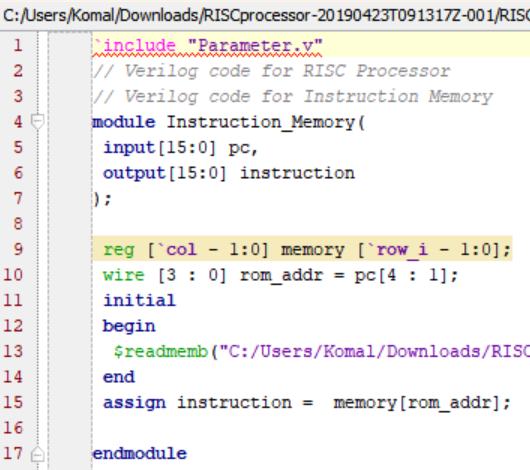
\includegraphics[scale=0.65]{Instruction_Mem}
\begin{center}
Verilog code for instruction memory
\end{center}

\vspace{5mm}
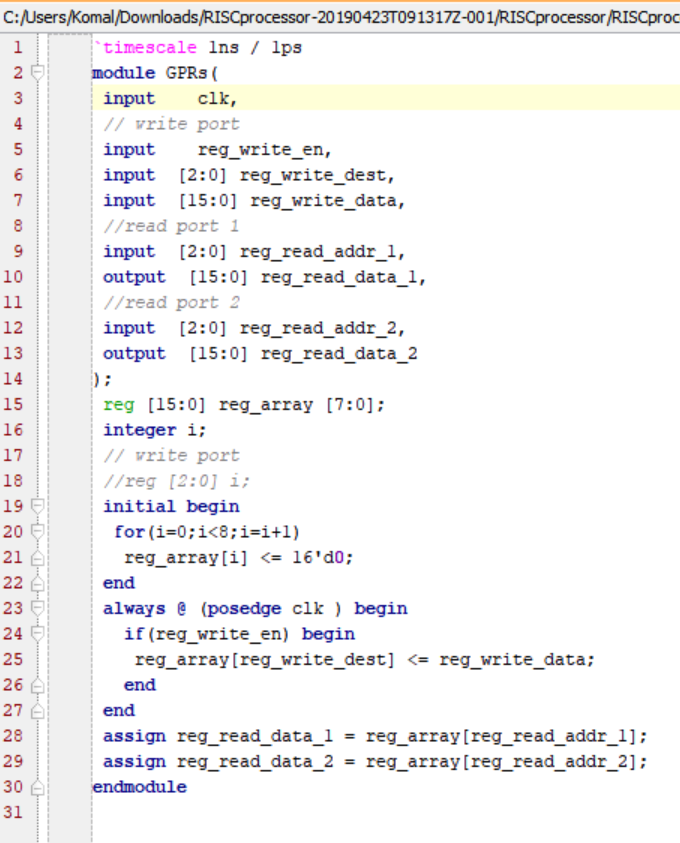
\includegraphics[scale=0.65]{GPR}
\begin{center}
Verilog code for register file
\end{center}

\vspace{5mm}
\includegraphics[scale=0.6]{Data_mem}
\begin{center}
Verilog code for data memory
\end{center}

\vspace{5mm}
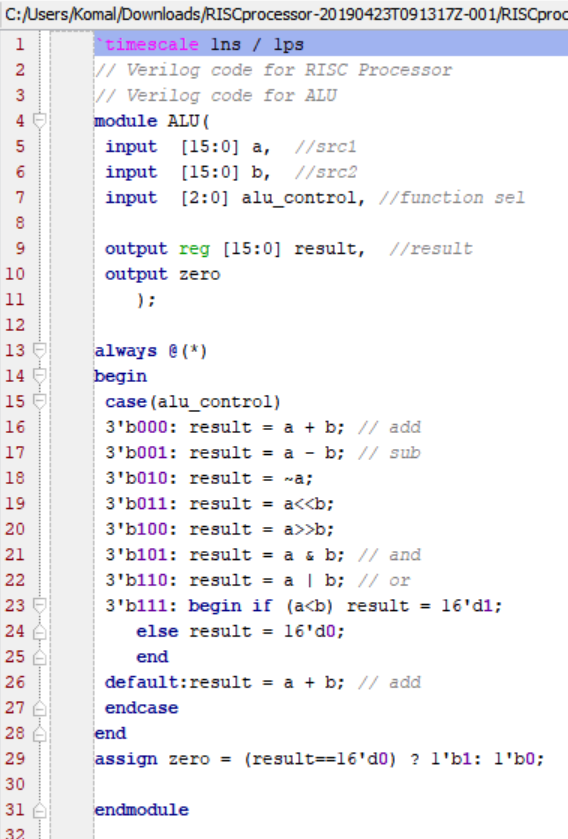
\includegraphics[scale=0.65]{ALU}
\begin{center}
Verilog code for ALU
\end{center}

\vspace{5mm}
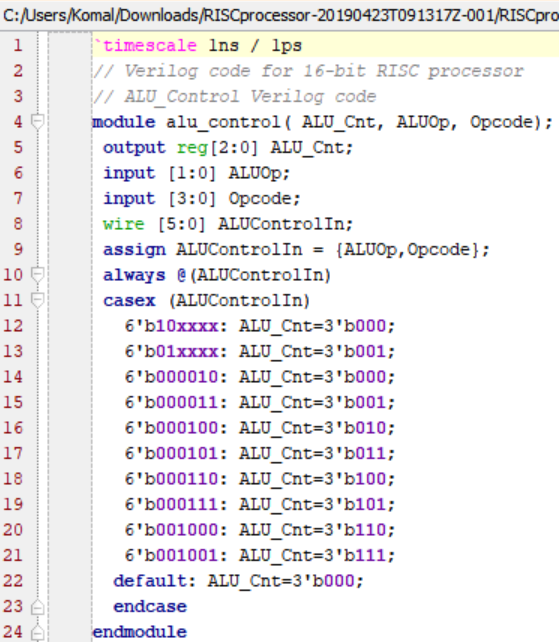
\includegraphics[scale=0.65]{ALU_CU}
\begin{center}
Verilog code for ALU Control Unit
\end{center}

\vspace{5mm}
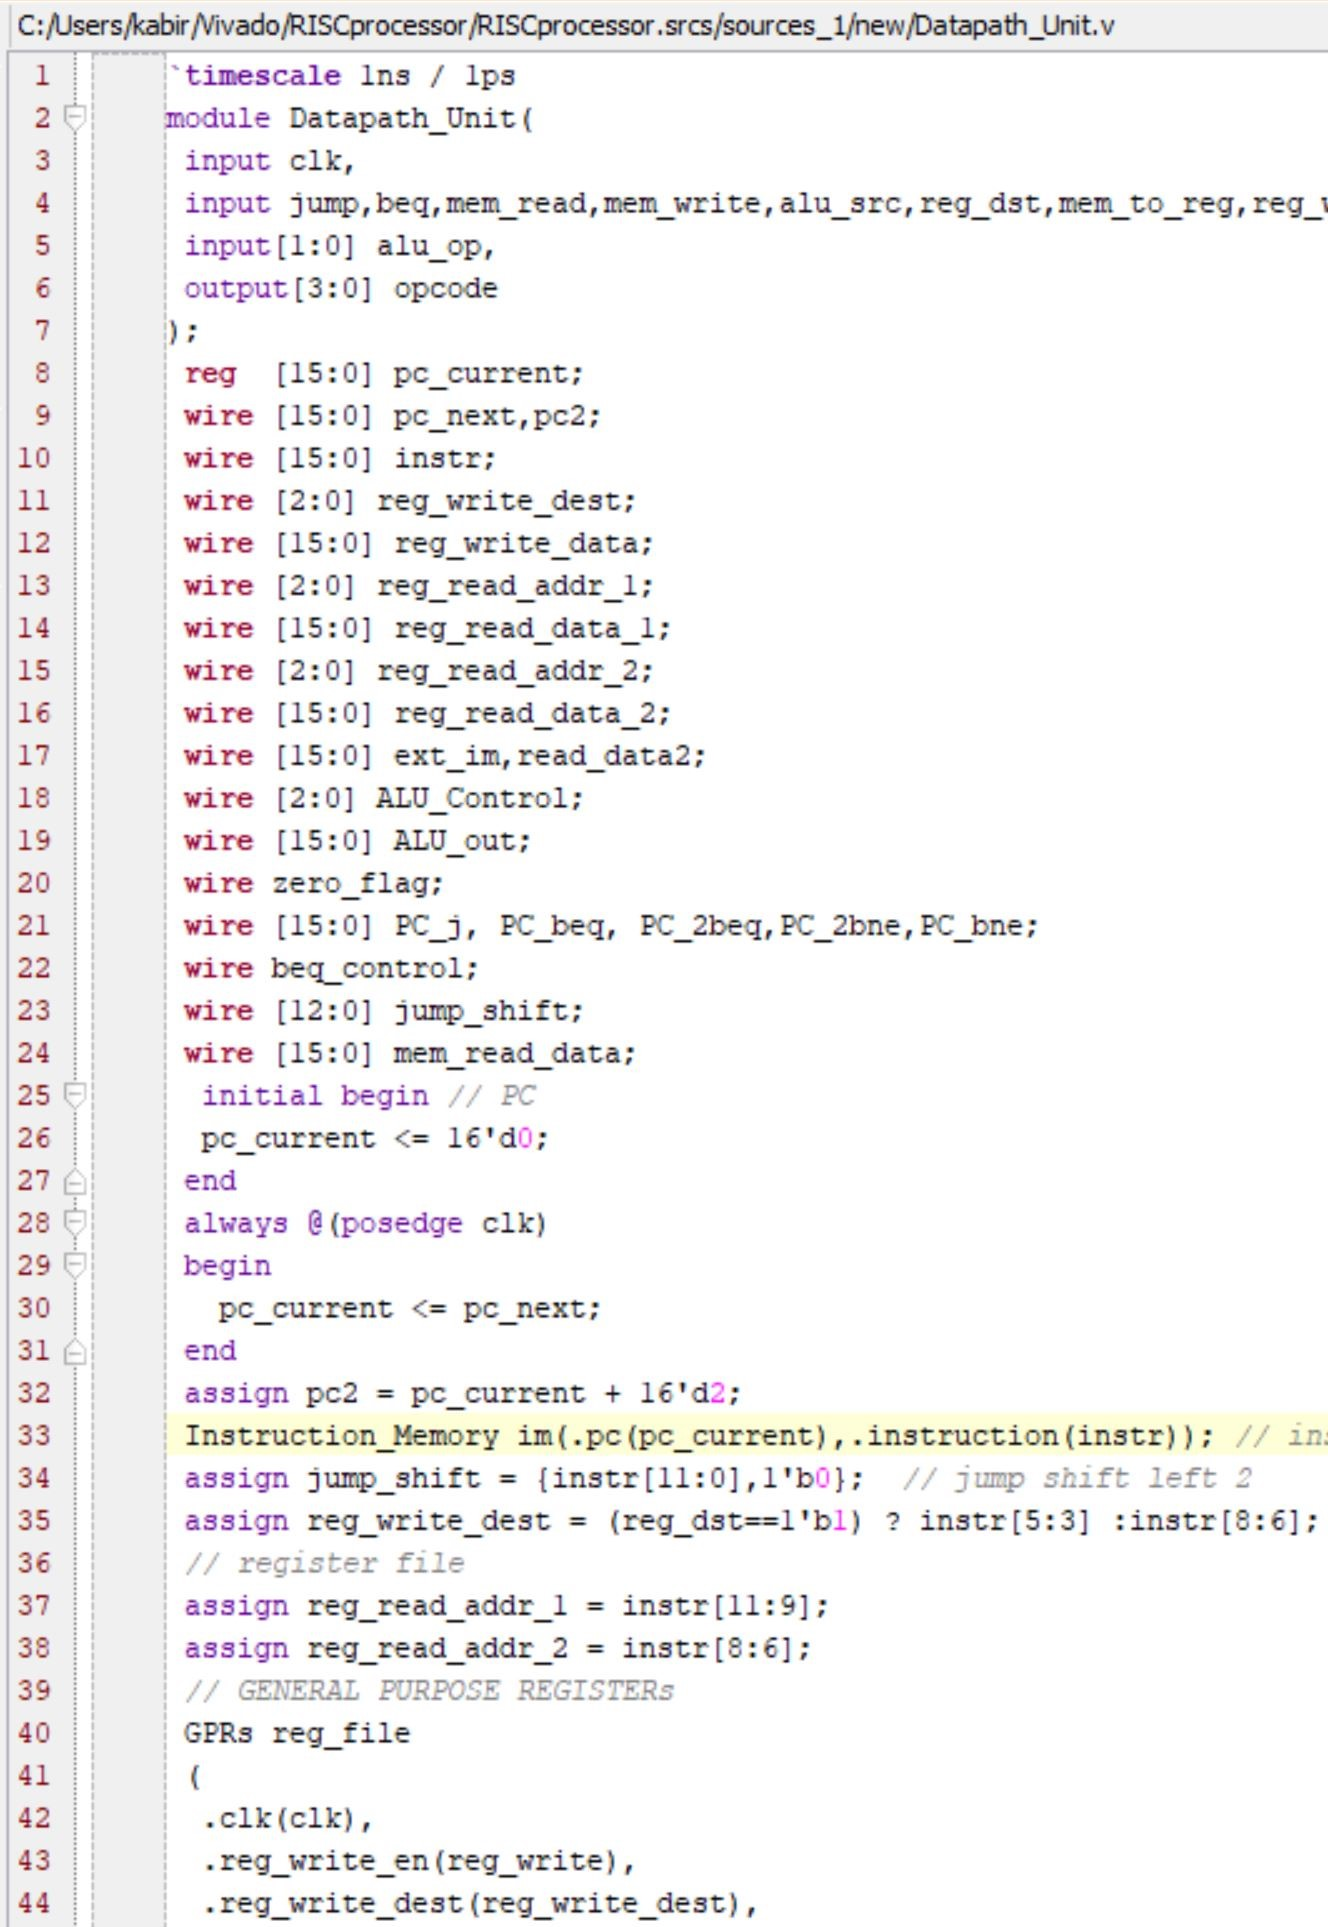
\includegraphics[scale=0.6]{Datapath_Unit(1)}
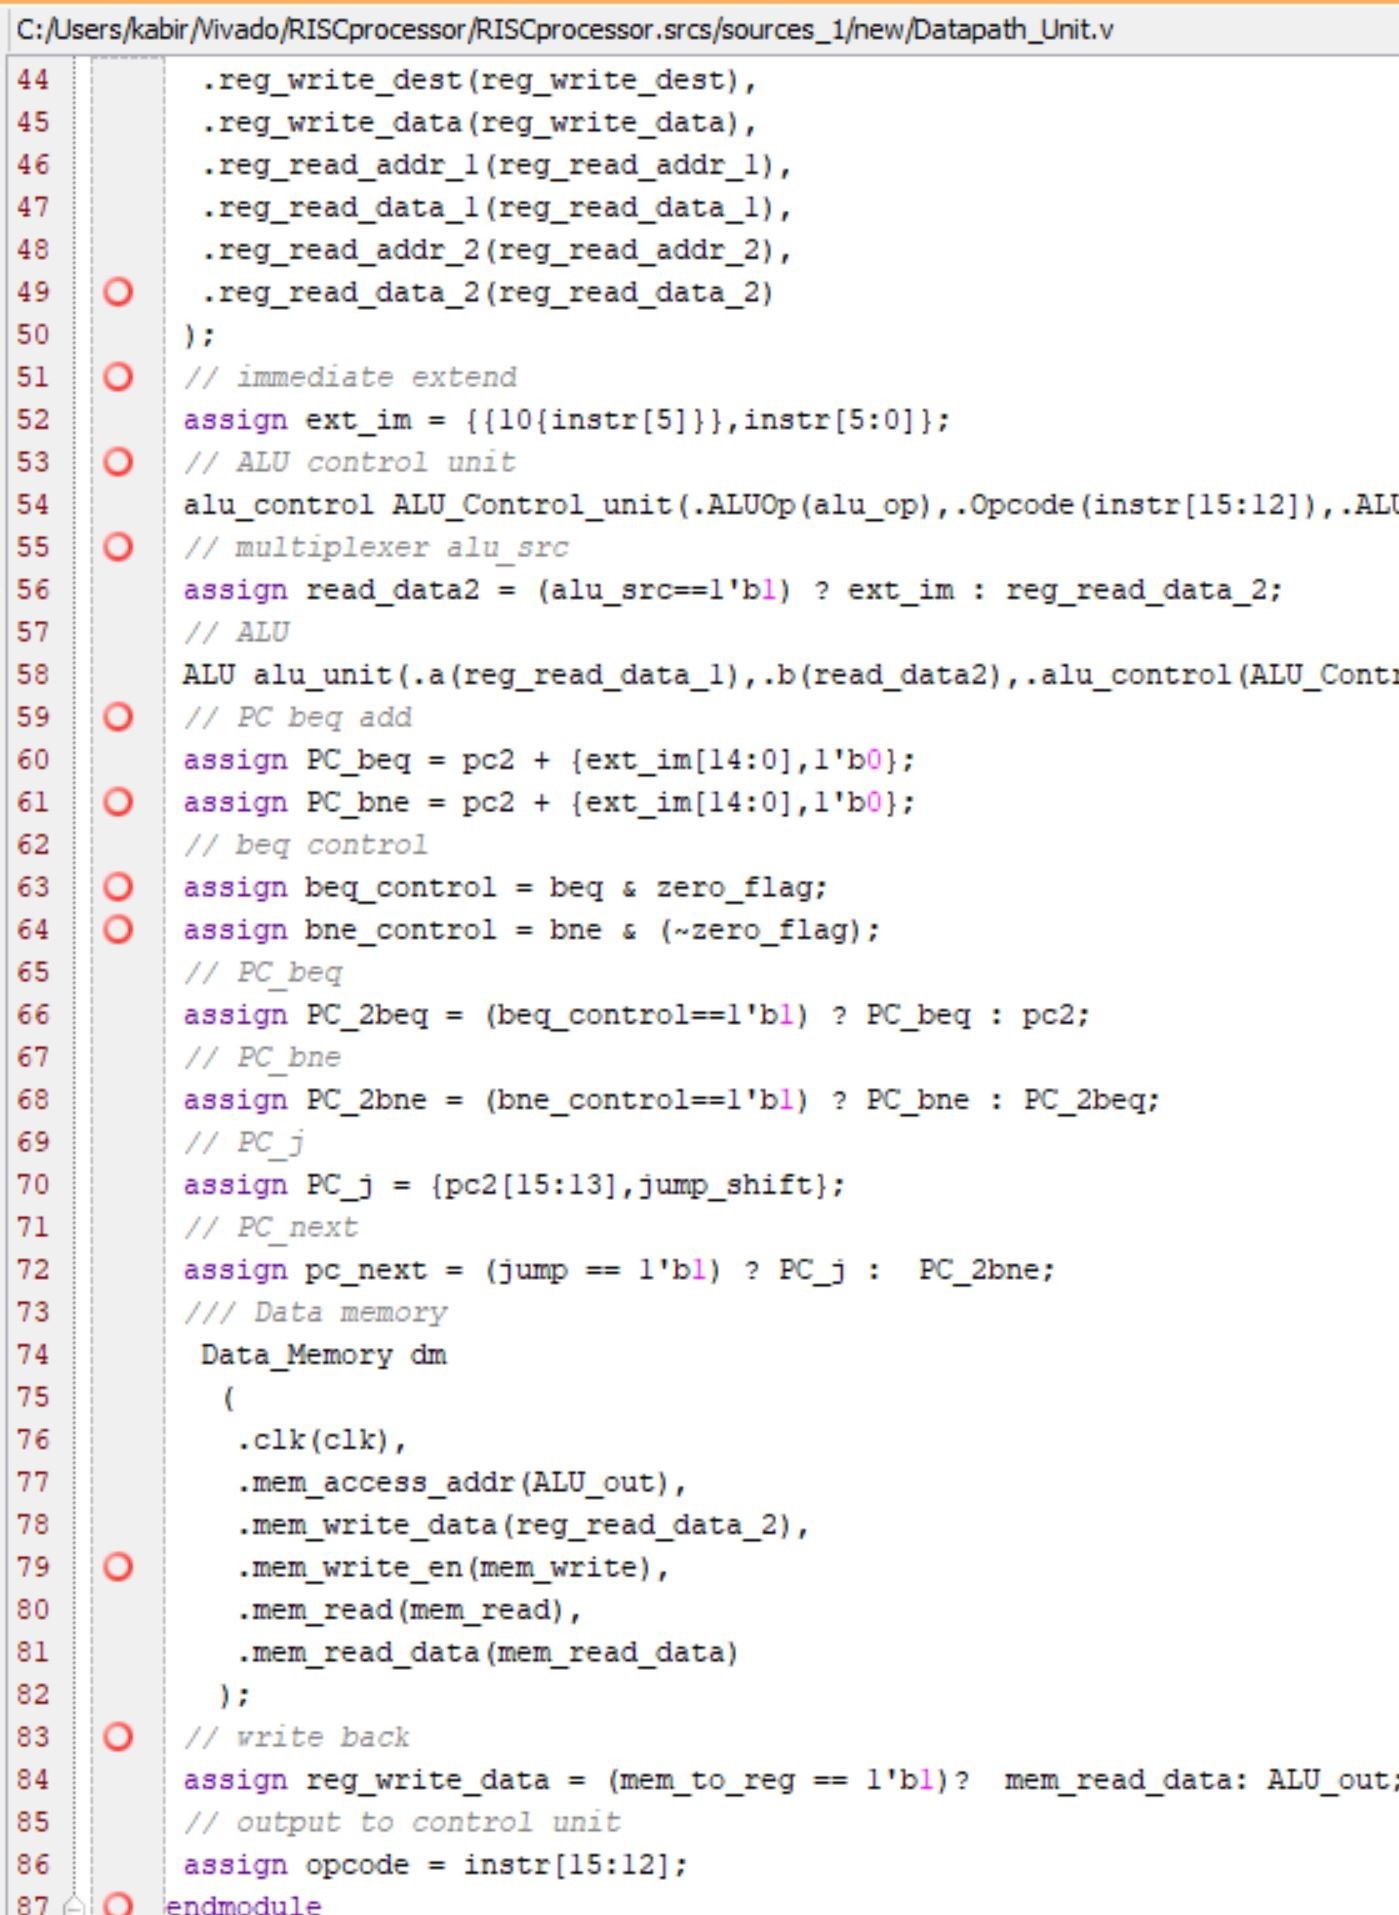
\includegraphics[scale=0.6]{Datapath_Unit(2)}
\begin{center}
Verilog code for data path of the processor
\end{center}

\vspace{5mm}
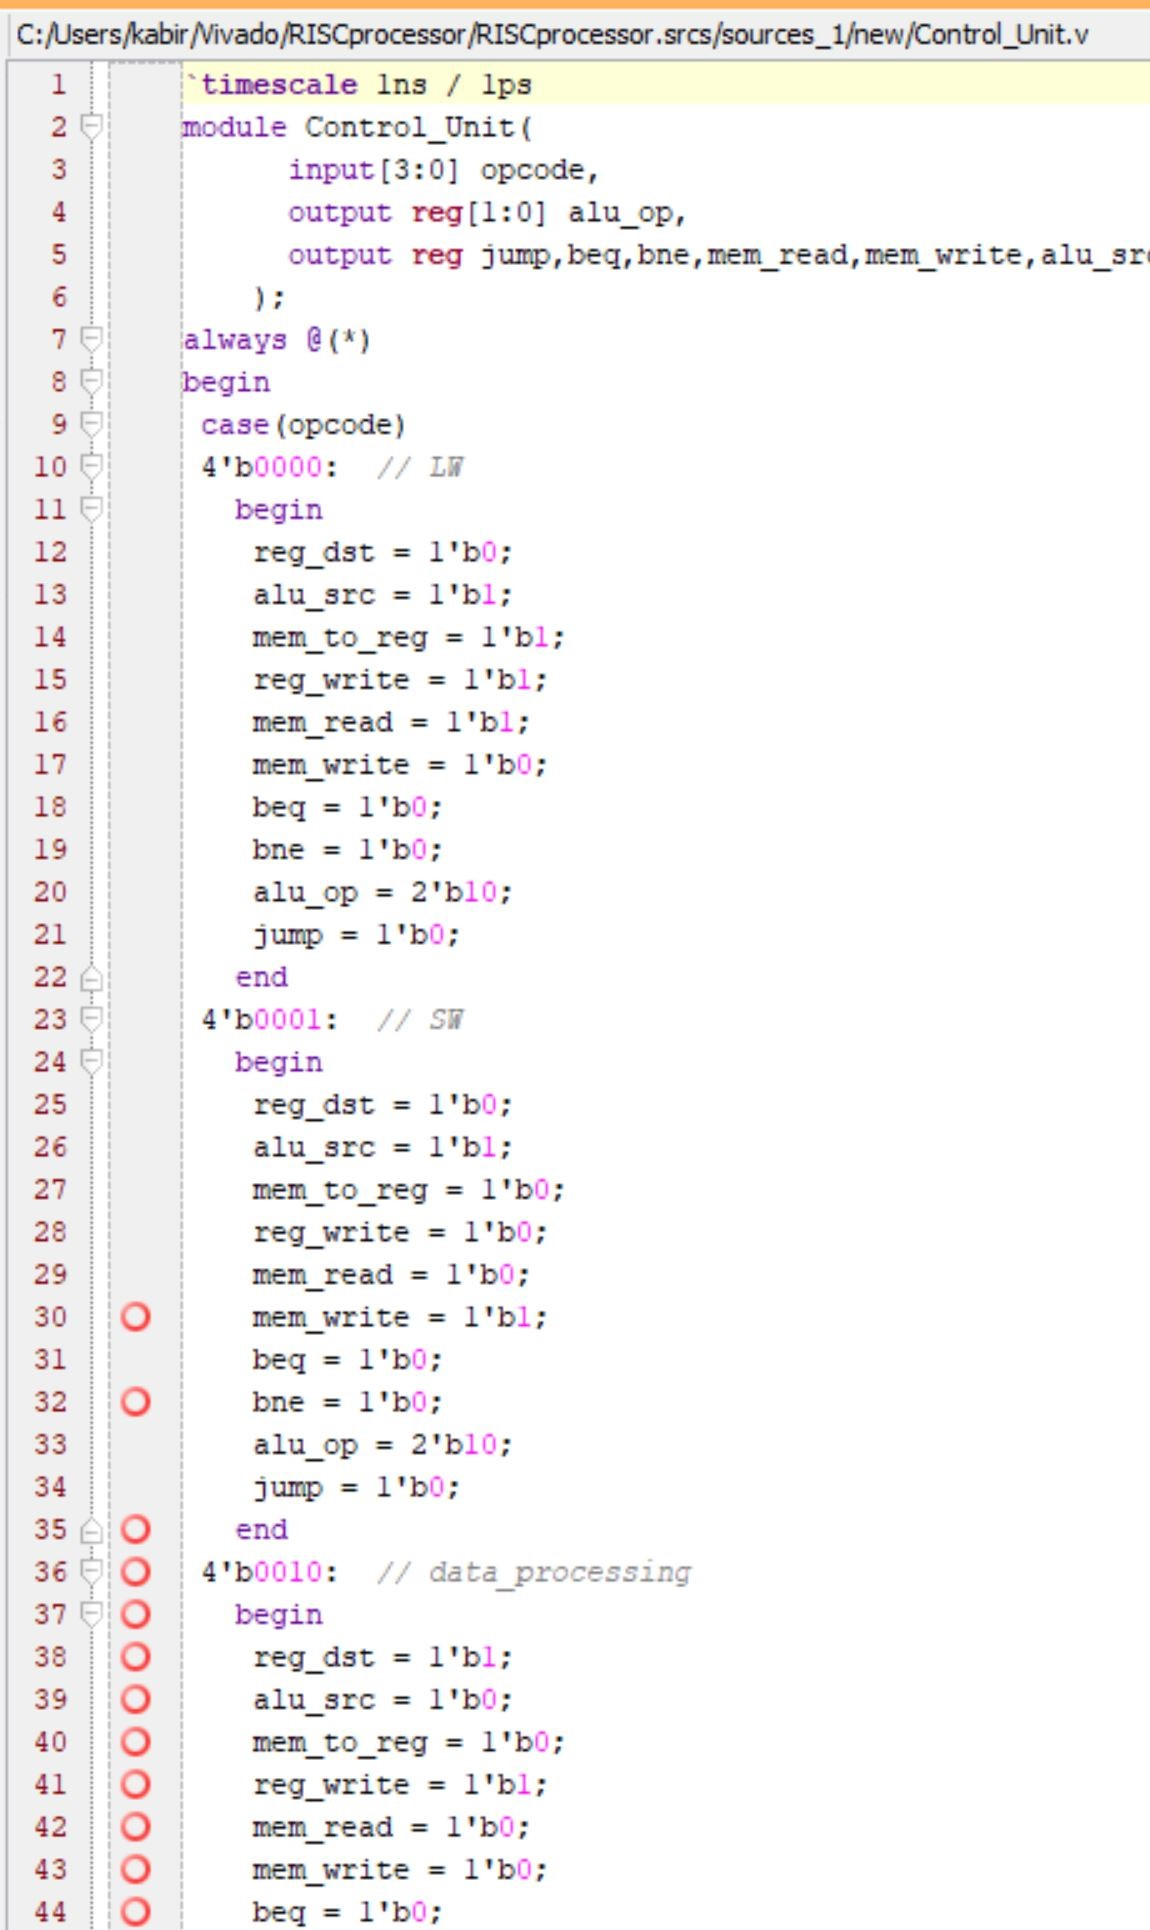
\includegraphics[scale=0.65]{Control_Unit(1)}
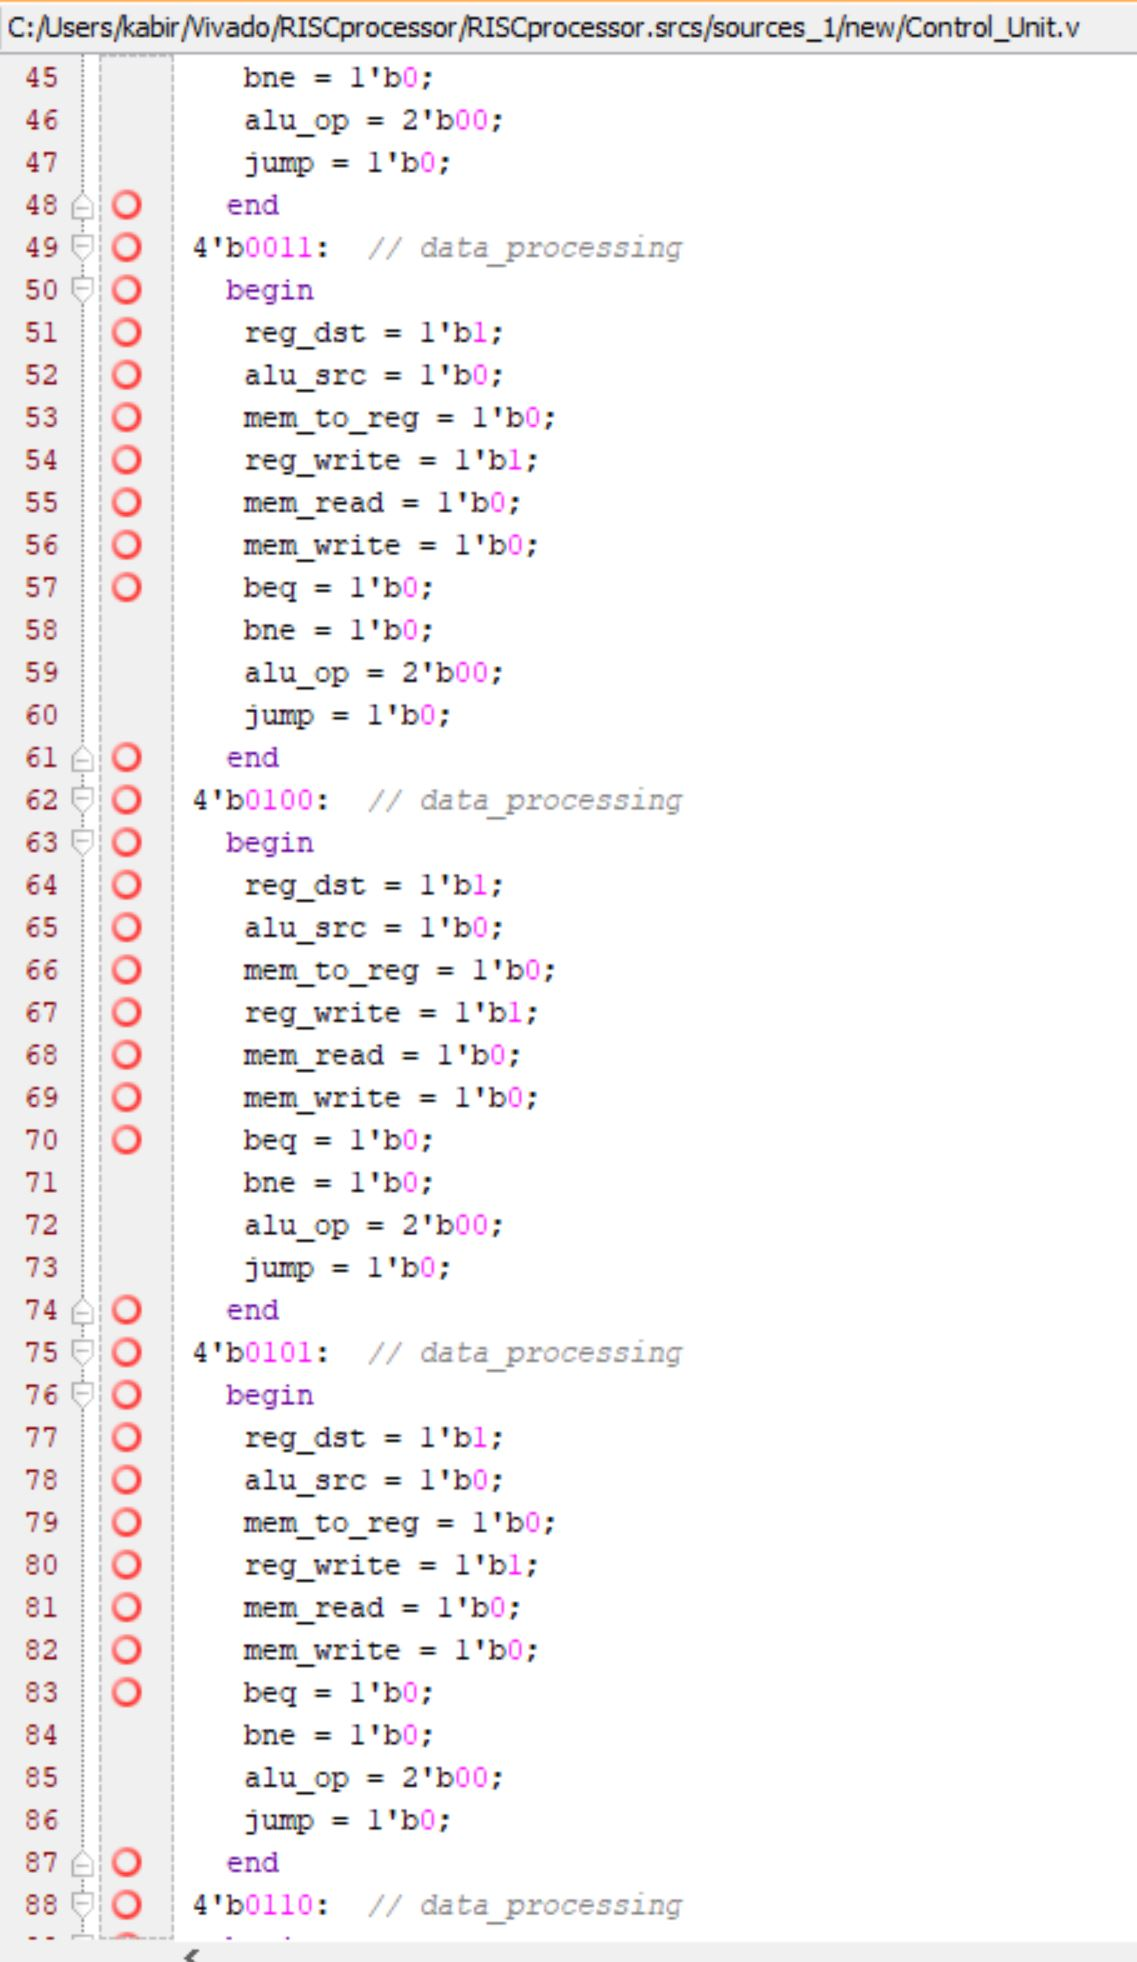
\includegraphics[scale=0.65]{Control_Unit(2)}
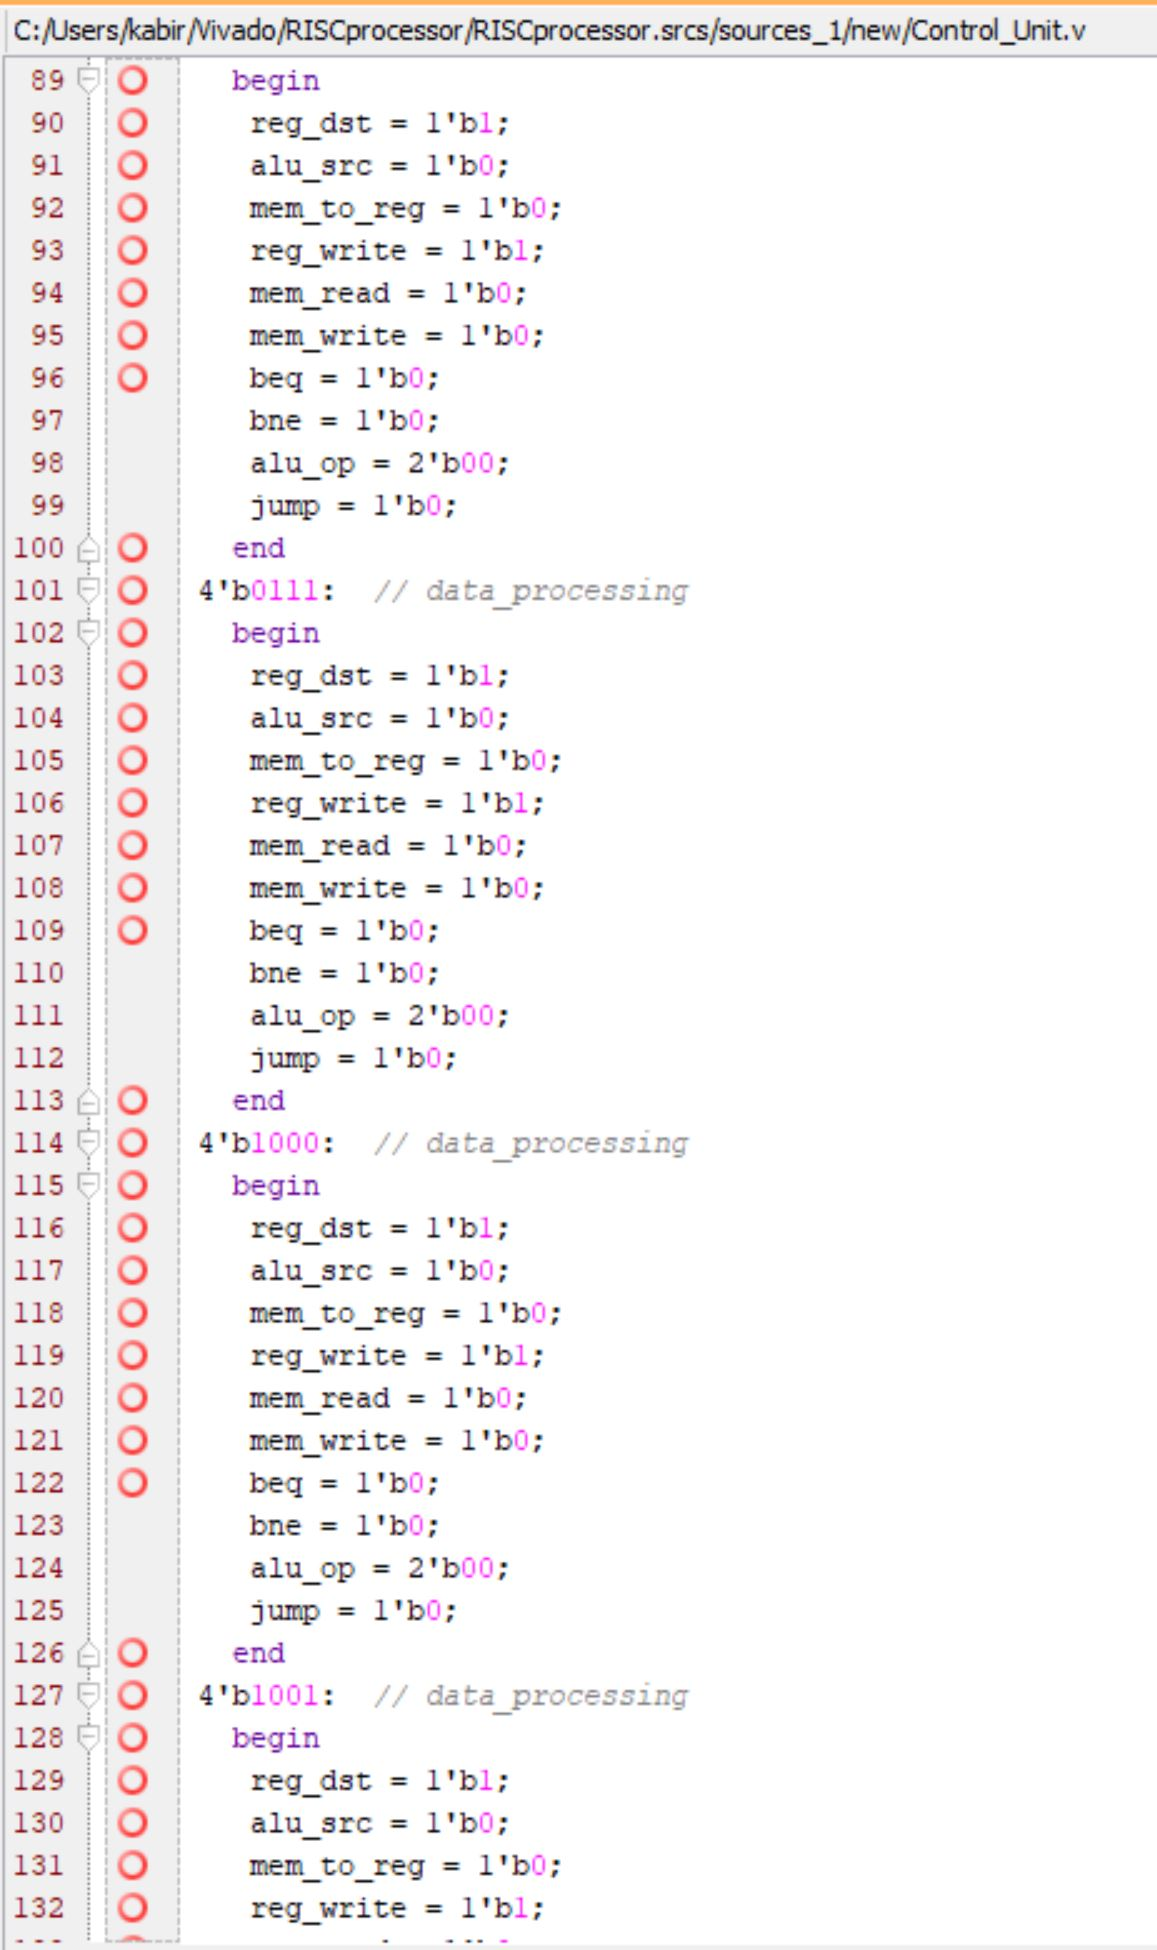
\includegraphics[scale=0.65]{Control_Unit(3)}
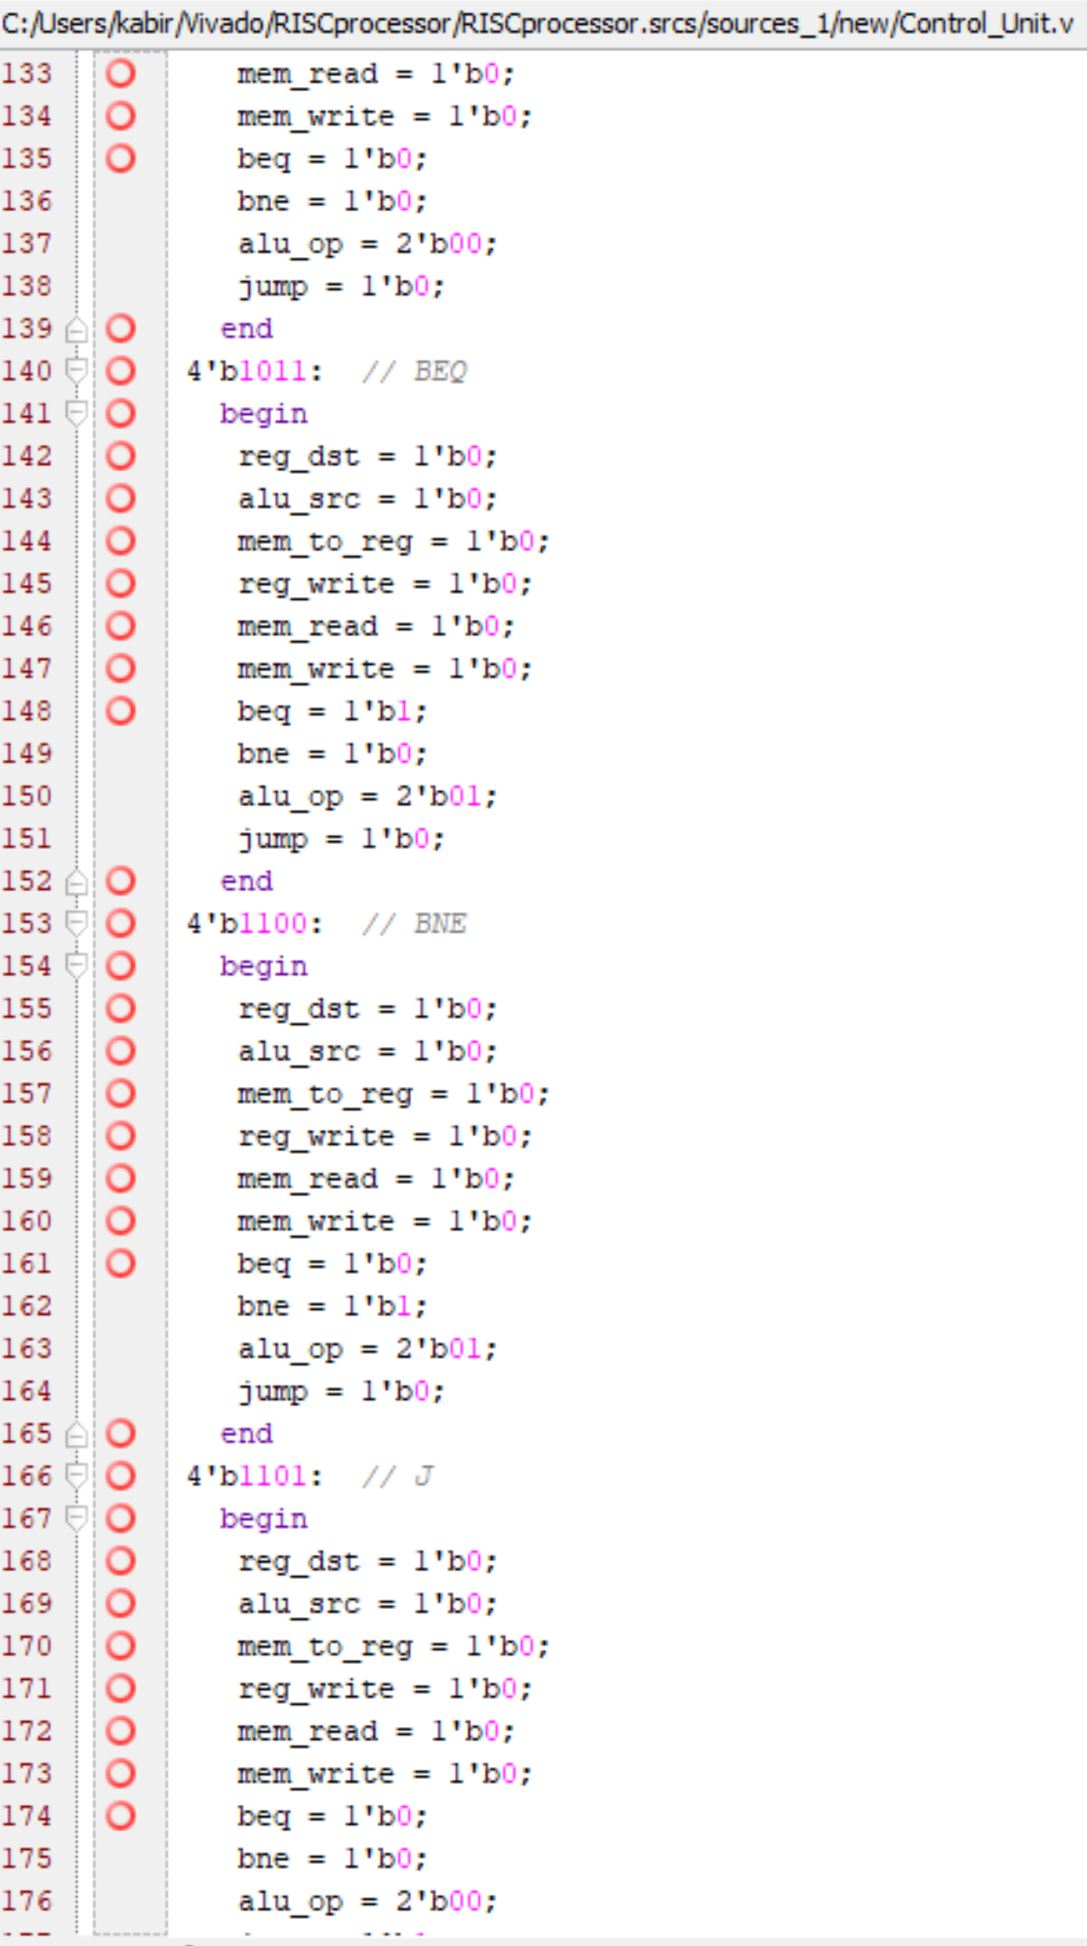
\includegraphics[scale=0.65]{Control_Unit(4)}
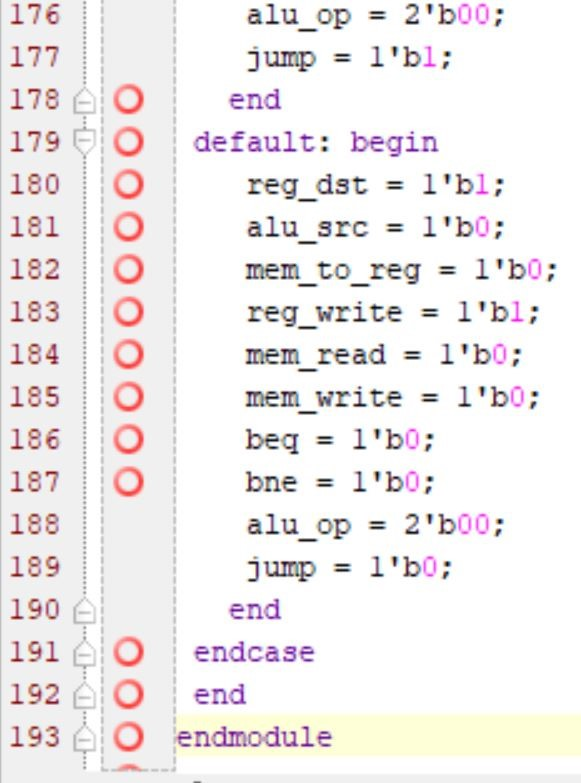
\includegraphics[scale=0.65]{Control_Unit(5)}
\begin{center}
Verilog code for Control Unit
\end{center}

\vspace{5mm}
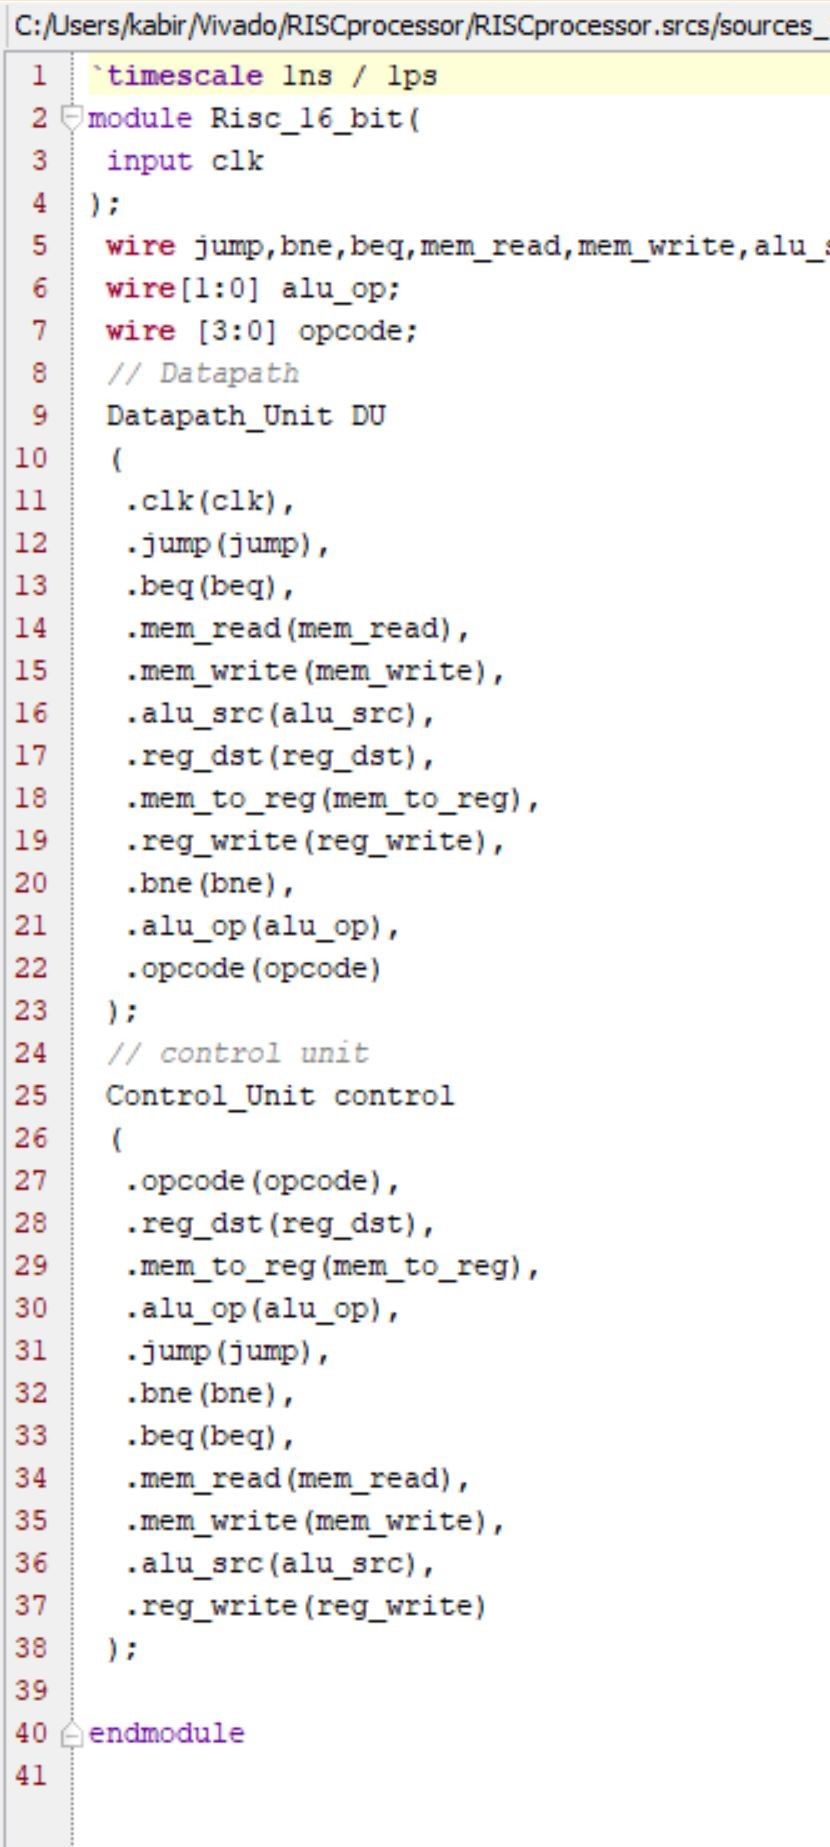
\includegraphics[scale=0.65]{Risc_16_bit}
\begin{center}
Verilog code for 16 bit RISC processor
\end{center}

\vspace{5mm}
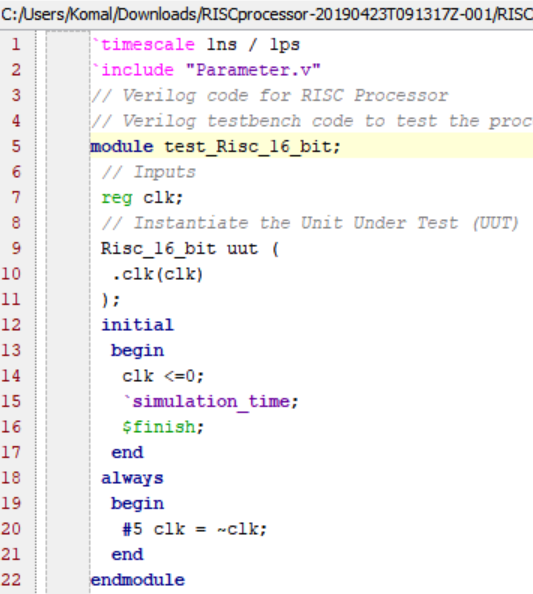
\includegraphics[scale=0.65]{test}
\begin{center}
Verilog code for testbench to test the processor
\end{center}

\vspace{5mm}
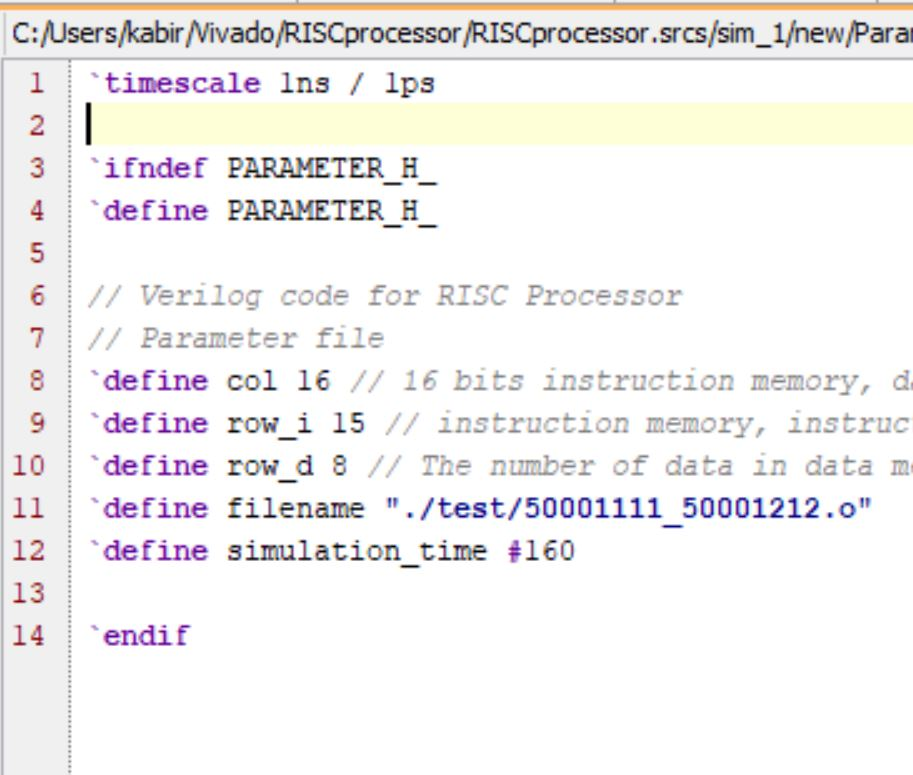
\includegraphics[scale=0.65]{Parameter}
\begin{center}
Verilog code for RISC processor Parameter file
\end{center}
\vspace{1mm}
\subsection{Simulation}
\vspace{2mm}
For the simulation, the following operations have been performed and results have been stored in registers ranging from R0-R7. R0 and R1 are used for simply loading data into it. R2 stores the result of the \textbf{ADD} operation on values contained in R0 and R1. Other such operations are \textbf{Subtraction, Bitwise AND, Bitwise OR, Set Less Than, Hamming distance (XOR)} and a \textbf{Jump} operation. \\

\vspace{5mm}
\includegraphics[scale=0.65]{inst_mem}
\begin{center}
Instruction memory file used for simulation
\end{center}

\vspace{5mm}
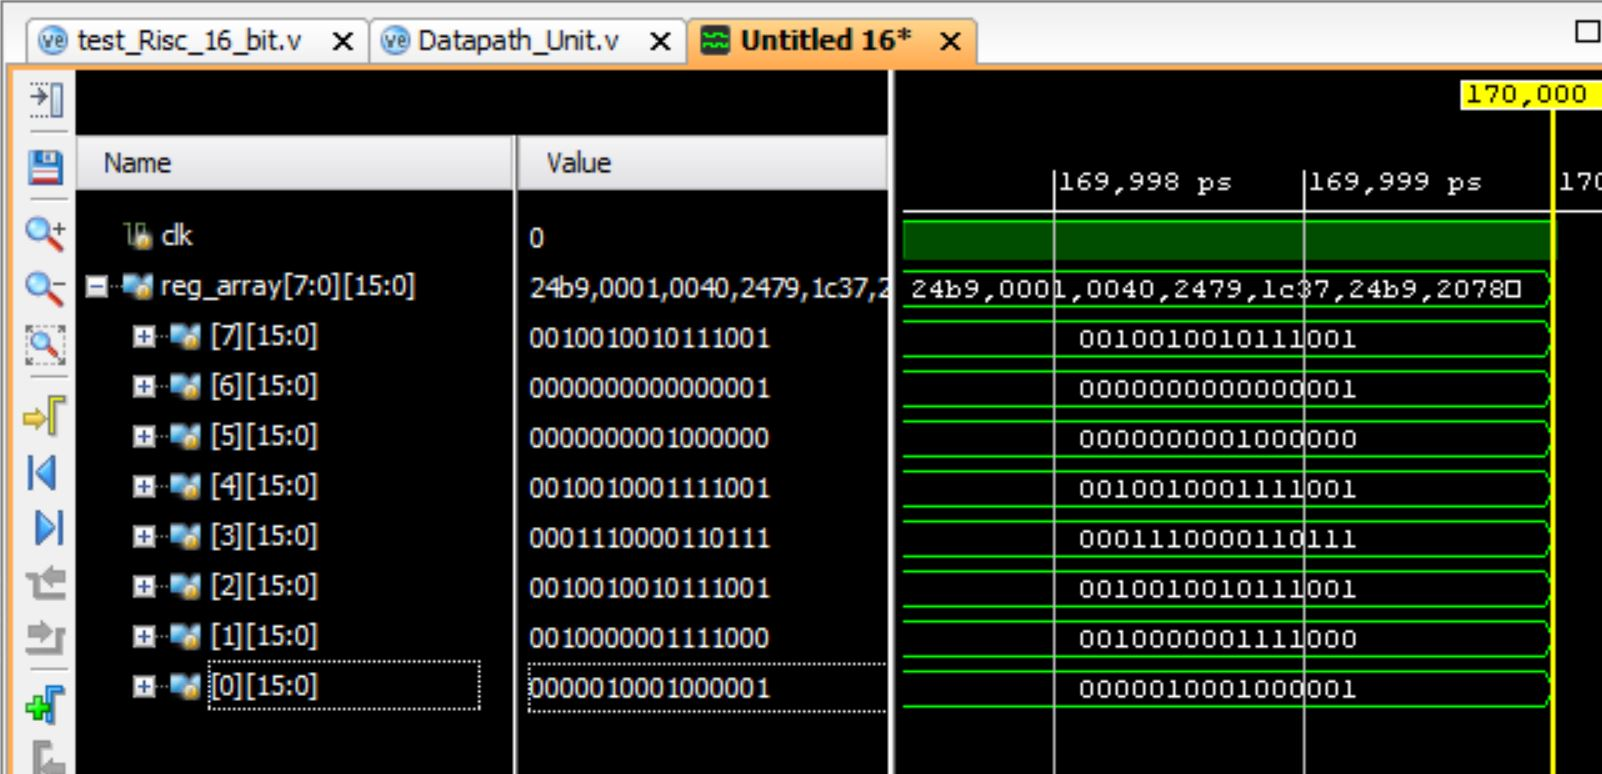
\includegraphics[scale=0.5]{Simulation(Binary)}
\begin{center}
Simulation Results (Binary)
\end{center}

\vspace{5mm}
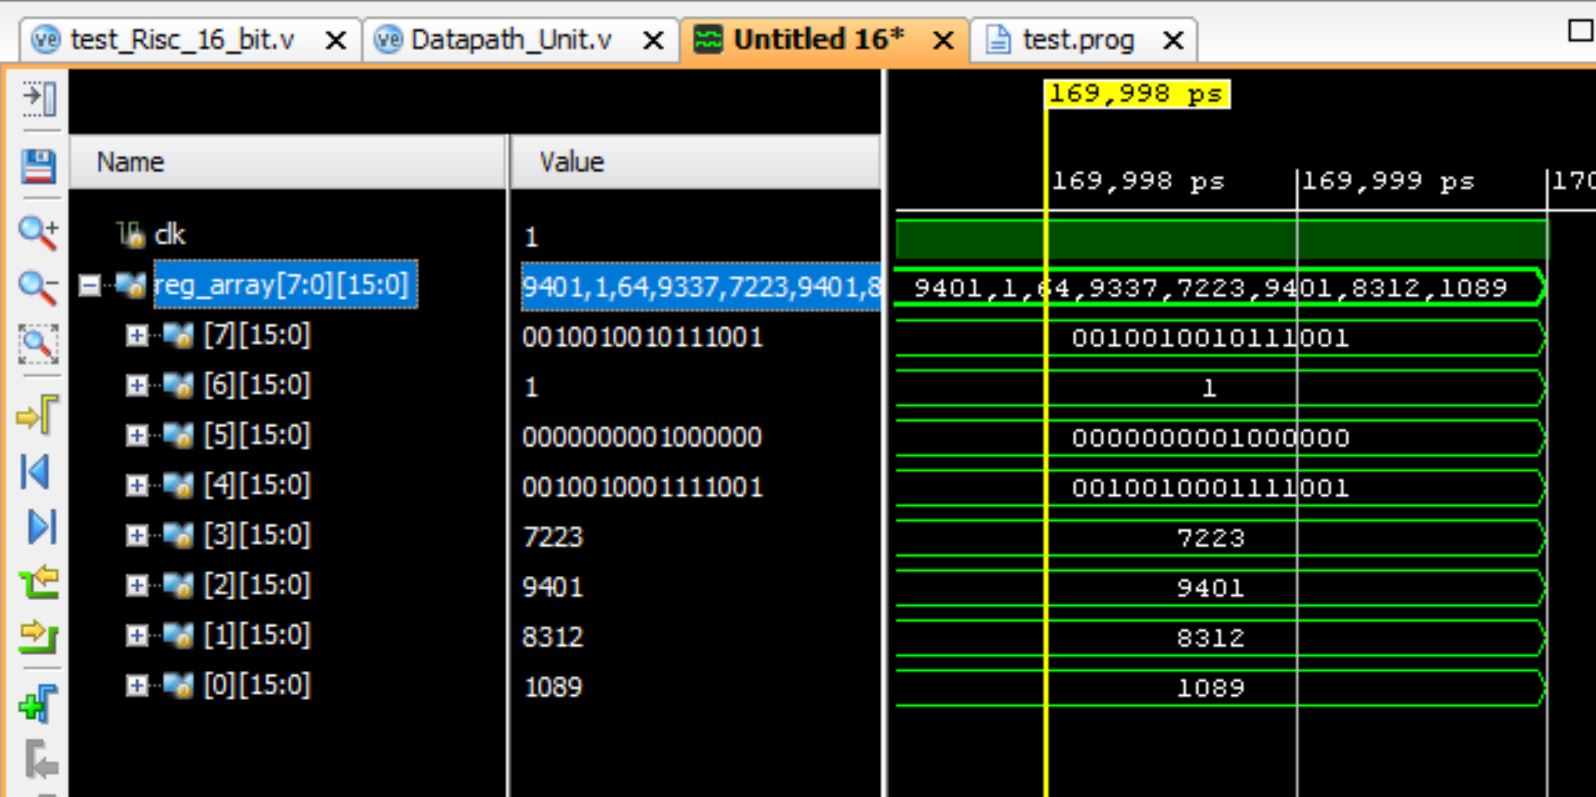
\includegraphics[scale=0.5]{Simulation(Decimal)}
\begin{center}
Simulation Results (Decimal)
\end{center}
\vspace{2mm}

\section{Conclusion}
Both are suitable at their own specific applications. Today, we use both RISC and CISC technology, and we call it \textbf{E.P.I.C} (Explicitly Parallel Instruction Computing)
 
Now we think of whether the RISC v CISC debate is still applicable today. It certainly was applicable in the 1980s and 90s when RISC came into the picture. This is what \textbf{David Patterson} had to say about it:
\begin{quote}
“Even a million transistors does not go far if a whole computer has to be built from it. That raises the question as to whether the extra hardware needed to implement CISC is the best way to use this ‘scarce’ resource”
\end{quote}

Of course, that was a million transistors, that was back then. Today, even an SoC (System on a chip) has got 6.9 BILLION transistors in it. Back then something that didn’t even give much of a result in terms of performance, like a branch predictor, was thought of as a big deal. Nowadays, almost all processors use efficient branch predictors that can predict if there’s a branch coming up in the next 10 to 20 instructions.
But here’s an interesting fact that most people don’t know. Starting with the Pentium Pro, Intel actually changed the way they designed their processors and this idea of a thing called Micro opt. What it does is that when it sees an instruction that says add one to this address in memory, it breaks it down into three separate instructions and sends those down the pipeline. So that means that today, a lot of CISC computers actually break down complicated commands in to RISC instructions. Intel added some extra logic at the beginning to split the variable length instructions into fixed length using brute force. That’s why x86 hasn’t been popular in smartphones, because the extra logic at the beginning actually produces extra heat and uses up more battery and is hence just not as power efficient as the ARM counterparts.

From our simulation, we observe that it was fairly easy to simulate a RISC processor as it has relatively simpler instruction formats and addressing modes. The same task would've been a much tougher ask had we tried to simulate a CISC processor due to the increased complexity of instructions and variable instruction size.

\vspace{10mm}
\section*{Acknowledgment}

Kabir Kanha Arora and Komal Talwar would like to thank their Computer Architecture teacher at Shiv Nadar University, \textbf{Dolly Sharma}, for the opportunity to engage in this endeavour. It was a fantastic learning experience and they are grateful for her guidance and constant support. They would also like to thank \textbf{Shaik Jani Babu}, a PhD student at Shiv Nadar University for sharing his knowledge of Verilog with them which proved to be very useful.

\begin{thebibliography}{00}
\bibitem{b1} Patterson, David A., and Carlo H. Sequin. "RISC I: A reduced instruction set VLSI computer." In Proceedings of the 8th annual symposium on Computer Architecture, pp. 443-457. IEEE Computer Society Press, 1981.

\bibitem{b2} Cocke, John, and Victoria Markstein. "The evolution of RISC technology at IBM." IBM Journal of research and development 34.1 (1990): 4-11.

\bibitem{b3} Hennessy, John L., and David A. Patterson. Computer architecture: a quantitative approach. Elsevier, 2011.

\bibitem{b4} Mano, M. Morris. Digital design. EBSCO Publishing, Inc., 2002.

\bibitem{b5} Blem, Emily, Jaikrishnan Menon, and Karthikeyan Sankaralingam. "Power struggles: Revisiting the RISC vs. CISC debate on contemporary ARM and x86 architectures." 2013 IEEE 19th International Symposium on High Performance Computer Architecture (HPCA). IEEE, 2013.

\bibitem{b6} Jamil, Tariq. "Risc versus cisc." Ieee Potentials 14.3 (1995): 13-16.

\bibitem{b7} Akram, Ayaz. "A Study on the Impact of Instruction Set Architectures on Processor’s Performance." (2017).

\end{thebibliography}
\end{document}